\documentclass[oneside,12pt,a4paper,headsepline,bibtotocnumbered]{memoir}
%\documentclass[oneside,12pt,a4paper]{memoir}
%\documentclass[a4paper,12pt,twoside,headsepline,pointlessnumbers,bibtotocnumbered]{scrbook}

\usepackage[utf8]{inputenc}
\usepackage{graphicx}
%\usepackage{lettrine}
\usepackage{hyperref}
\usepackage{color}
\usepackage{url}

\usepackage[T1]{fontenc}
\usepackage{lmodern}
%\usepackage{psfig}
%\usepackage{psfrag}
%\usepackage{epsfig}
\usepackage{epstopdf}
% Formato de paquetes de SCTP y NALUs de SVC...
%\usepackage{bytefield}
% Algoritmos
%\usepackage{algorithm}
%\usepackage{algpseudocode}
% Columnas
\usepackage{multicol}
\usepackage[labelfont=bf]{caption}
% Listados
\usepackage{listings}
\usepackage{pdfpages}
\usepackage{indentfirst}
%euro
%\usepackage{eurosym}

%\usepackage[bookmarks = true, colorlinks=true, linkcolor = black, citecolor = black, menucolor = black, urlcolor = black]{hyperref}

%\newsubfloat{figure}% Allow subfloats in figure environment

%\usepackage{wrapfig}

\usepackage{listings}
%\usepackage[usenames,dvipsnames]{xcolor}

\definecolor{gray97}{gray}{.97}
\definecolor{gray75}{gray}{.94}
\definecolor{gray45}{gray}{.45}
\definecolor{verde}{RGB}{230,255,204}

\usepackage{listings}

\newcommand\Tstrut{\rule{0pt}{2.6ex}}       % "top" strut
\newcommand\Bstrut{\rule[-0.9ex]{0pt}{0pt}} % "bottom" strut
\newcommand{\TBstrut}{\Tstrut\Bstrut} % top&bottom struts


\newenvironment{filecode}[1][]
  {\minipage{\linewidth}% \begin{filecode}[#1]
   \lstset{basicstyle=\ttfamily\footnotesize,frame=single,#1}}
  {\endminipage}% \end{filecode}


%\DeclareInputText{128}{\euro}

\definecolor{azulillo}{rgb}{0.8,0.85,1}
\definecolor{marronrp3}{rgb}{.9,.9,.7}
\definecolor{salmon}{rgb}{1,.9,.8}
\definecolor{rojo}{rgb}{.8,0.1,.0}
\definecolor{rojo2}{rgb}{.6,0.3,.2}

\lstset{
  basicstyle=\ttfamily,
  columns=fullflexible,
  showstringspaces=false,
  commentstyle=\color{gray}\upshape
}

\lstdefinelanguage{XML}
{
  morestring=[b]",
  morestring=[s]{>}{<},
  morecomment=[s]{<?}{?>},
  stringstyle=\color{black},
  identifierstyle=\color{darkblue},
  keywordstyle=\color{cyan},
  morekeywords={xmlns,version,type}% list your attributes here
}

\lstdefinestyle{BashInputStyle}{
  language=bash,
  basicstyle=\small\sffamily,
  numbers=left,
  numberstyle=\tiny,
  numbersep=3pt,
  frame=tb,
  columns=fullflexible,
  linewidth=0.9\linewidth,
  xleftmargin=0.1\linewidth,
  commentstyle=\color{dkgreen},
}

\definecolor{dkgreen}{rgb}{0,0.6,0}
\definecolor{gray}{rgb}{0.5,0.5,0.5}
\definecolor{mauve}{rgb}{0.58,0,0.82}

\lstset{frame=tb,
  language=Java,
  aboveskip=3mm,
  belowskip=3mm,
  showstringspaces=false,
  columns=flexible,
  basicstyle={\small\ttfamily},
  numbers=none,
  numberstyle=\tiny\color{gray},
  keywordstyle=\color{blue},
  commentstyle=\color{dkgreen},
  stringstyle=\color{mauve},
  breaklines=true,
  breakatwhitespace=true
  tabsize=3
}


\def\changemargin#1#2#3{\list{}{\rightmargin#2\leftmargin#1\headsep#3}\item[]}
\let\endchangemargin=\endlist


%\configuracion{TituloDocumento}{TextoEncabezadoIzdo}
\newcommand{\configuracion}[2]{
	\renewcommand{\shorthandsspanish}{}
	\title{#1}
	\date{}
	\evensidemargin -6mm  \oddsidemargin -0.4cm \textwidth 16.7cm
	\usepackage[colorlinks=true,linkcolor=blue,urlcolor=blue]{hyperref}
	\textheight 24cm \topmargin -0.65cm
	\pagestyle{fancy}
	\lhead{#2}
	\rhead{\thepage}
	\cfoot{}
}

\newcommand{\escudos}{
	\begin{changemargin}{-1.0cm}{-3cm}{0cm}
		\begin{flushleft}
  			\begin{figure}
    			
\includegraphics[scale=0.2]{escudo.jpg}
    			\hspace*{8cm}
    			\includegraphics[scale=0.45]{informatica.png}
    		\end{figure}
		\end{flushleft}
	\end{changemargin}
}

\newcommand{\asignatura}[1]{
	\begin{center}
#1
	
	\end{center}
}

\newcommand{\titulacion}[1]{
	\begin{center} 
	#1
	\end{center} 
}

\newcommand{\cursiva}[1]{
	\textit{#1}
}

\renewcommand{\bibname}{References}

%%%%%%%%%%%%%%%%%%%%%%%%%%%%%%%%%%%%%%%%%%%%%%%%%%%%%%%%%
% \shadowbox{Texto}: Marco sombreado. 
%\ovalbox{Texto}: Marco ovalado. 
%\doublebox{Texto}: Marco doble. 
% \Ovalbox{Texto}. Marco ovalado. 


% \cajaBorde {texto}{color letra}{color fondo}
\newcommand{\cajaBorde}[3]{
	\noindent
	\fcolorbox{#2}{#3}{
  		\begin{minipage}[t]{.96\linewidth}
   			 \vspace{.05cm}
    		\begin{center}
     			 \vspace{.1cm}
     			#1
   			 \end{center}
 		 \end{minipage}
	}
}

%caja{texto}{color caja}{espacio superior}{espacio inferior}
\newcommand{\caja}[4]{
	\colorbox{#2}{
 	 \begin{minipage}[t]{.96\linewidth}
 	 \vspace{#3}
  		
			#1
		
   	 \vspace{#4}
 	 \end{minipage}
	}
}

\newcommand{\borde}[1]{\framebox{#1}}

%\portada{asignatura}{pratica}{tituloCaja}{titulacion}{autores}
\newcommand{\portada}[5]{
	%PORTADA
	\thispagestyle{empty}

	%Escudo universidad
	\escudos

	\LARGE

	\asignatura{#1}

	\vspace*{0.8cm}

	\begin{center}
		\textbf{#2} %Práctica 1\\
	\end{center}


	\begin{center}

		
	\colorbox{azulillo}{
 	 	\begin{minipage}[t]{.96\linewidth}
 	 		\vspace{.5cm}
  		
			\begin{center}
				\textbf{#3}
			\end{center}
		
   	 		\vspace{.02cm}
 		\end{minipage}
	}		
		
	\end{center}

	\Large
	\vspace {3cm}

	\titulacion{#4}

	%Fecha
	\begin{center}
		\today
	\end{center}
	\normalsize
	\vspace*{2cm}

	\begin{flushright}
		#5
	\end{flushright}

}

%\portada{asignatura}{pratica}{tituloCaja}{titulacion}{autores}
\newcommand{\portadaumu}[5]{
	%PORTADA
	\thispagestyle{empty}
\setlength{\unitlength}{1 cm} %Especificar unidad de trabajo
\thispagestyle{empty}
\begin{picture}(18,4)
\put(0,0){
\includegraphics[scale=0.33]{escudo.jpg}}
\put(11.5,0){\includegraphics[scale=0.43]{informatica.png}}
\end{picture}
\\
\\
\begin{center}
\textbf{{\Huge University Charles III}\\[0.5cm]
{\LARGE Faculty of Computer Science}}\\[1.25cm]
\Large #1\\[2cm]


\LARGE \textbf{#3}\\[0.3cm]

{\large #5}\\[1.6cm]
#4\\[1cm]
Madrid - \today
\end{center}

}

\newcommand{\indice}{

	\newpage
	\setcounter{page}{1}
	\renewcommand{\thepage}{\roman{page}}
	\tableofcontents
	\newpage
	\clearpage
	\setcounter{page}{1}
	\renewcommand{\thepage}{\arabic{page}}
}


\lstset{basicstyle=\small\ttfamily,showstringspaces=false,language=sh,frame=tb,columns=fullflexible}

% Separación entre párrafos
%\setlength{\parindent}{0pt}
% %\nonzeroparskip

% Veelo un poco cambiado

\makeatletter
\newlength{\numberheight}
\newlength{\barlength}
\makechapterstyle{myveelo}{%
\setlength{\beforechapskip}{40pt}
\setlength{\midchapskip}{25pt}
\setlength{\afterchapskip}{40pt}
\renewcommand{\chapnamefont}{\normalfont\LARGE\flushright}
\renewcommand{\chapnumfont}{\normalfont\HUGE}
\renewcommand{\chaptitlefont}{\normalfont\HUGE\bfseries\flushright}
\renewcommand{\printchaptername}{%
\chapnamefont\MakeUppercase{\@chapapp}}
\renewcommand{\chapternamenum}{}
\setlength{\numberheight}{18mm}
\setlength{\barlength}{\paperwidth}
\addtolength{\barlength}{-\textwidth}
\addtolength{\barlength}{-\spinemargin}
\renewcommand{\printchapternum}{%
\makebox[0pt][l]{%
\hspace{.4em}%
\resizebox{!}{\numberheight}{\chapnumfont \thechapter}%
%\hspace{.8em}%
%\rule{\barlength}{\numberheight}
}}
\makeoddfoot{plain}{}{}{\thepage}
}
\makeatother

% Configuración de márgenes más anchos
\setmarginnotes{0pt}{0pt}{0pt}
\settypeblocksize{675pt}{450pt}{*}
\setlrmarginsandblock{2.7cm}{2.7cm}{*}
\setulmarginsandblock{2.7cm}{2.7cm}{*}
\checkandfixthelayout
\raggedbottom

\chapterstyle{myveelo}

% Numeración de subsecciones
\setcounter{secnumdepth}{2}

\newcommand{\first}[2]{
%lhang=1, nindent=0pt, 
	\lettrine[lines=3]{#1}{#2}%
}

\newcommand{\figura}[4]{%
    \begin{figure}[ht]
    \begin{center}
	    \includegraphics[#2]{#1}
	    \caption{#3}
	    \label{#4}
    \end{center}
    \end{figure}
}


\begin{document}
	
	\newcommand{\HRule}{\rule{\linewidth}{0.5mm}}

\begin{titlingpage}
\begin{center}
 
% Upper part of the page
\vfill

\includegraphics[scale=1.2]{./images/escudo}\\[3em]
\textsc{\LARGE Universidad Carlos III de Madrid}\\[0.5cm]
\textsc{\Large Trabajo de Fin de Grado}\\[0.5cm]

% Title
\HRule \\[0.6cm]
\textbf{\Large Integration of CROWD SDN-based DMM solution with NI PXI Systems for LTE emulation}
\HRule \\[0.6cm]
 
% Author and supervisor
\begin{minipage}{0.45\textwidth}
\begin{flushleft} \large
\emph{Student:}\\
Jason \textsc{Moorcroft}\\ jmoorcr@it.uc3m.es
\end{flushleft}
\end{minipage}
\begin{minipage}{0.45\textwidth}
\begin{flushright} \large
\emph{Tutor:} \\
Antonio \textsc{De la Oliva}\\
aoliva@it.uc3m.es
\end{flushright}
\end{minipage}
 
\vfill
 
% Bottom of the page
{\large \today}
 
\end{center}

\end{titlingpage}
	
	%Acknowledgments:
\textsc{\Large Acknowledgments}\\[0.5cm]


This project marks the end of an amazing part of my life, I wouldn't have been able to achieve it without the help of many people.\\

First of all, thanks to my family for supporting me the whole way and making  me feel like anything with hard work can be achieved. Thanks to those words, I have found the strength to not give up even when I thought I wasn't capable of accomplishing what I set out to do.\\

To my partner Maria, thank you so much for making this journey by me, for being there to help me without asking and for making this stage of my life as amazing as it has been. \\

To "Mis Costillas", for making those long afternoons in the library and in class so much more interesting. For the amazing places we have visited throughout these years, thank you.\\

Thank you to my friends for being understanding and helping me disconnect from the long days at university and show me a good time.\\

Thanks to my tutors,Pablo and Carlos, for guiding me through this project and showing interest in helping me express my ideas.\\
















	
	
	\clearpage{\cleardoublepage}
	
	\makepagestyle{init}
	   \makeevenfoot{init}{\thepage}{}{}
	   \makeoddfoot{init}{}{}{\thepage}
	   \makeevenhead{init}{}{}{}
	   \makeoddhead{init}{}{}{}
	   \makeheadrule{init}{0pt}{0pt}
	
	\pagestyle{init}
	  \tableofcontents*\thispagestyle{init}
	  \clearpage
	  \listoffigures*\thispagestyle{init}
	  \clearpage
	  \listoftables*\thispagestyle{init}
	
  	\chapter*{Abstract}
\addcontentsline{toc}{chapter}{Abstract}

The lack of expertise that people have on how to perform a good training session, leads to inefficiency and bad practices that can lead people to quit or injure themselves. With the cost to have a personal trainer or somebody to manage a persons training session being very high, there is an opportunity to improve the user experience with automated services that provide relevant information and keeps track of the progress that is being made.\\

This project implements a trainer chat bot that alleviates the cost of having a personal trainer, but maintaining many of the features they would provide. Over the years chat bots have steadily been incorporated into society, the flexibility and cost chat bots have, makes a very lucrative option for monotonous operations such as some provided by a personal trainer. 






	\clearpage

	\pagestyle{ruled}
  
  	\chapter{Introduction}\label{chap:1}
Technology and the impact it is having in our society is changing the way we think and the way we interact with each other. With more and more automation in the workplace many monotonous jobs are disappearing and more creative ones are replacing them. This and the fact that technology has opened the mind and ability for people to start a business as the cost to startup a business thanks to technology has greatly reduced.
The objective of this project is to automate the personal training area as it has been relatively untouched. The problem is that many people unknowingly train in a way that in the long term may cause them injury, this is due to the lack of knowledge and guidance to train differently and safely. Gym trainers may provide some guidance but with the amount of people normally in these gyms they can’t be always there to help. The idea is to create a chatbot that can aid, track progress and create training sessions that adapt to each user whenever the user needs them. 
\section{Background}\label{sec:chap1_background}
Machine Learning (ML) algorithms in recent years have improved greatly thanks to the immense computing power available. This with the amount of data currently accessible, has naturally led the way for the development of bots that can communicate with people, originally with basic phrases and over time in a more complex and natural manner. New technologies have made it more intuitive and easier to work on this area with many Natural Language Processing (NLP) libraries such as Natural Language Tool Kit (NLTK) that help translate human spoken phrases to something easier for the computer to understand. Other libraries like TensorFlow or Scikit-Learn provide functionality to train models based on the processing done in NLTK.
Nowadays, even though the libraries mentioned before are still frequently used, it is more common now to see platforms that abstracts the users from the inner workings of the algorithms and instead leaves the user with an intuitive UI for the user to create their own functionality for the chatbot.

Thanks to the access we have now to smartphones and social platforms the integration of chatbots in these platforms is growing steadily as it allows the user to communicate with help centers without waiting a long time to get a response.

\section{Motivation}\label{sec:chap1_moti}
The motivation to develop this project comes from the time-consuming activity of preparing a time table with what muscles and exercises to train and the forgetful way of tracking a person’s progress when going to the gym, for this reason, with the knowledge acquired over the years and the technology available this project came to life. It is not only a project to finish the degree it is a project that after giving it in will still be worked on over time to add more functionality and make it a truly useful application that can be used by users outside the University environment. This will be more of a proof of concept to verify the viability of further developing and investing the time to add more functionality.

\subsection{Survey}\label{sec:chap1_reas_app}

To prove that the application has a market opportunity an inquire was made to a group of people with over 200 people, the results where interesting as will be explained below. The language of the form is in Spanish as the public inquired live in Spain.\\

As shown below most of the users filling the form are from age 16 to 25, this gives context to some of the answers given afterwards, in this case generational mentality plays an important role as different age groups may have a different opinion on gym training. In this case the target group even though available for every age group is more focused on people in those age limits as they are the most common at gyms, the least informed and the more friendly with technology they are.

\begin{center}
	\begin{figure}[h!]
		\centering
		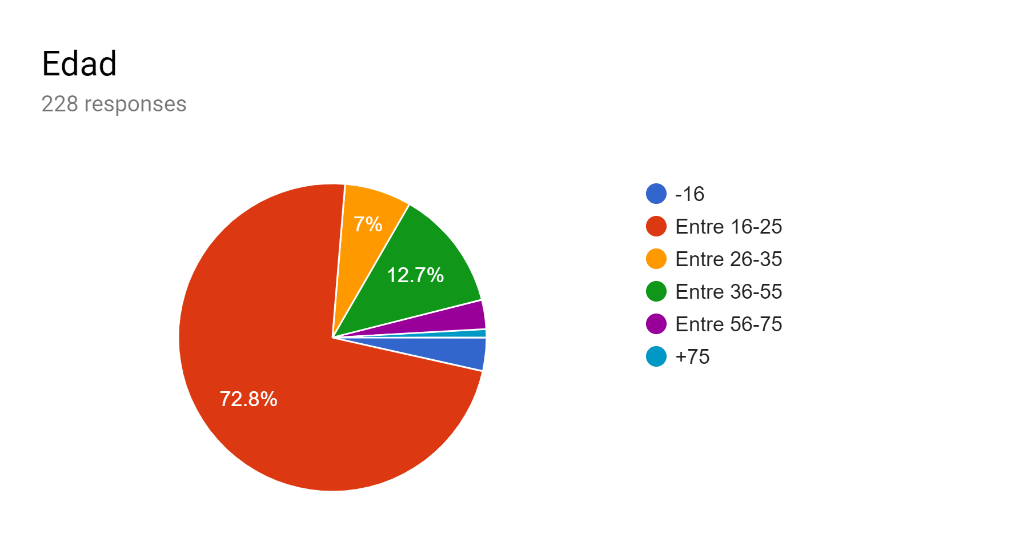
\includegraphics[scale=1]{./images/4-age}
		\caption{Survey: Age}
		\label{4_age}
	\end{figure}
\end{center}

In the case of gender, the pool has been varied with close to 50\% of each gender, this with the age group gives a general perception of what people think of the questions asked.

\begin{center}
	\begin{figure}[h!]
		\centering
		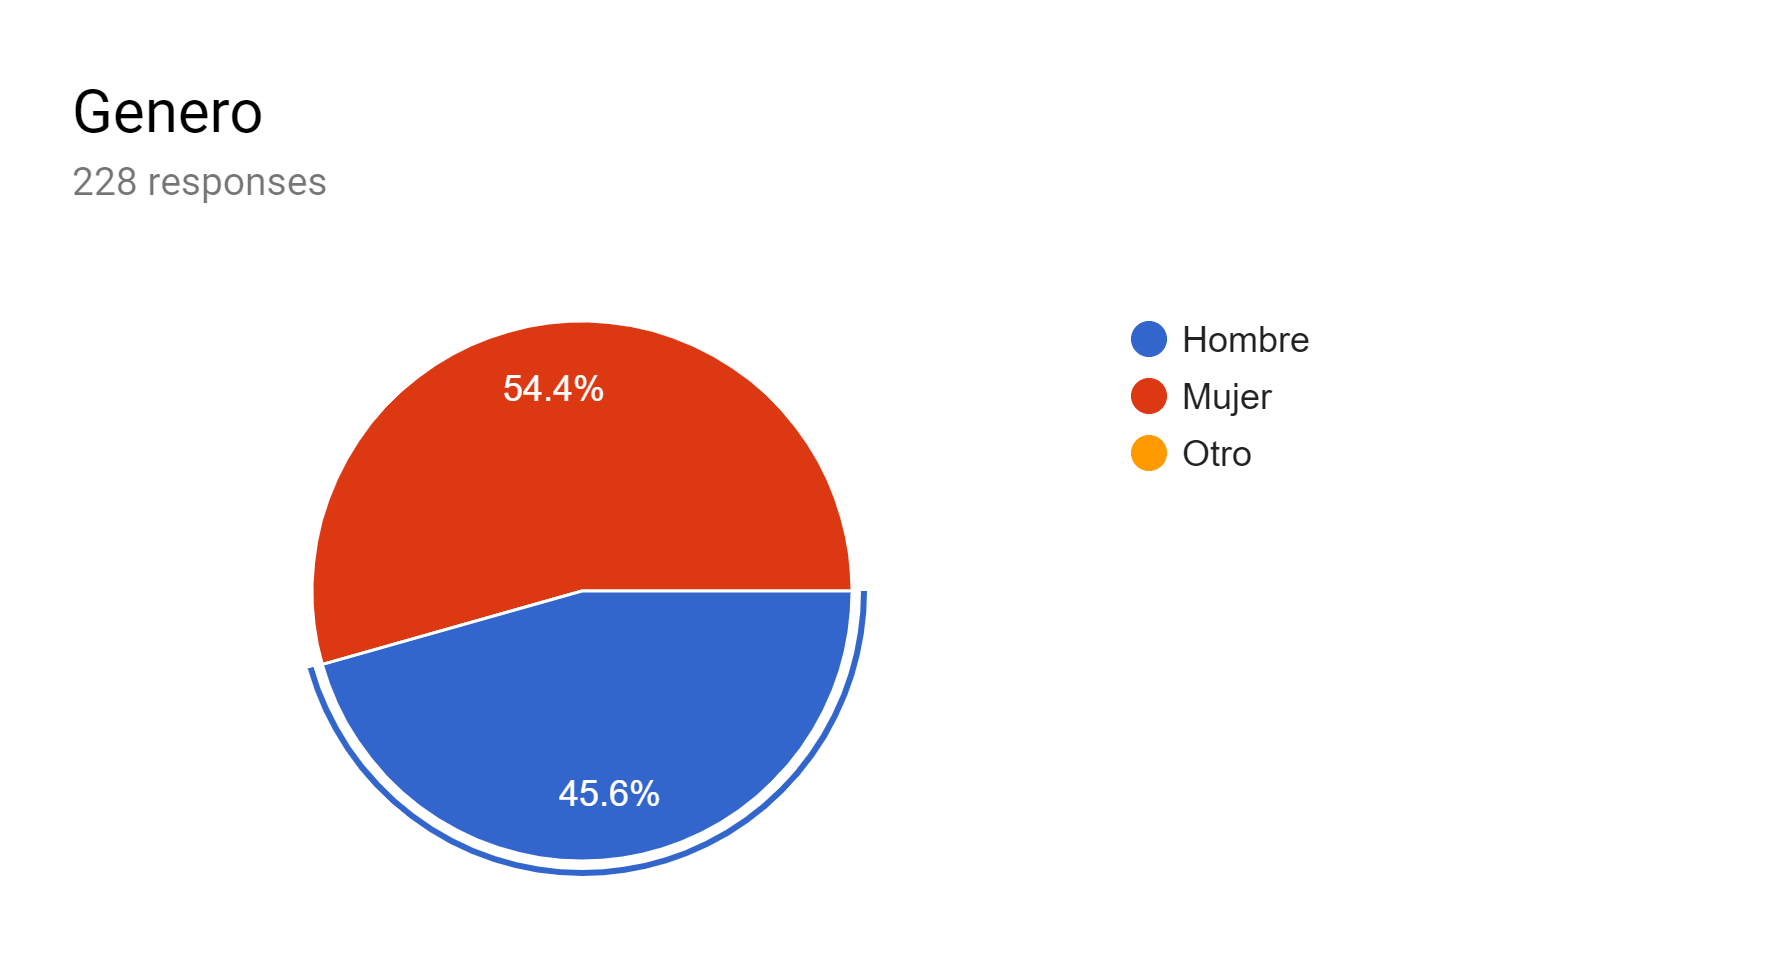
\includegraphics[scale=0.25]{./images/4-genero}
		\caption{Survey: Gender}
		\label{4_genero}
	\end{figure}
\end{center}

The following graph starts to show some interesting results, we can see that 30\% of the people asked don’t do any type of training and a sum of 24,1\% only train one to two times a week, this isn’t unexpected but that is over 50\% of people that train below the recommended amount weekly.

\begin{center}
	\begin{figure}[h!]
		\centering
		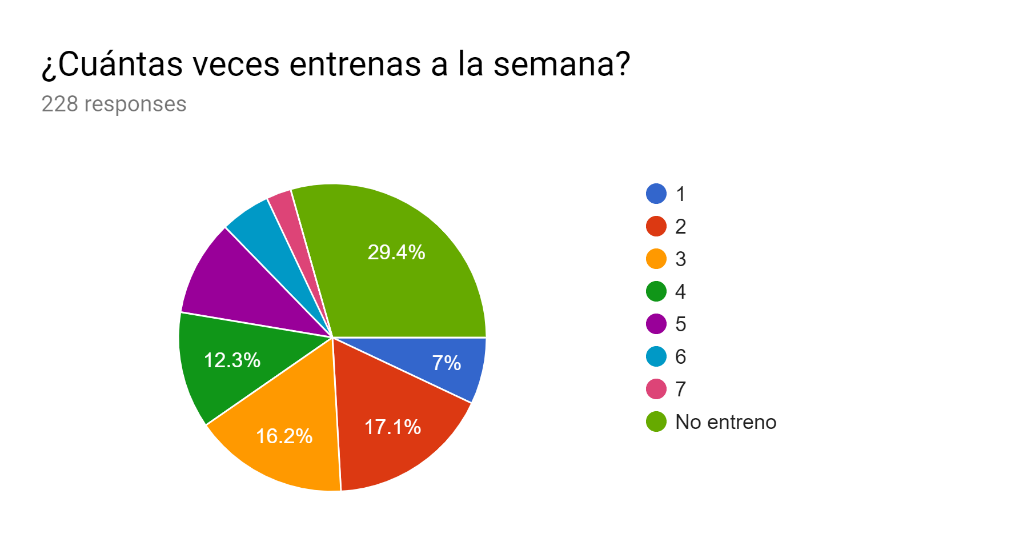
\includegraphics[scale=1]{./images/4-exe-freq}
		\caption{Survey: Gym Frequency}
		\label{4_exe_freq}
	\end{figure}
\end{center}

In the next graph the conclusions we can extract is that from the people that did the survey 30,7\% follow their own knowledge when going to the gym, this is something that is very frequent in gyms and it is the main source of dropouts as many people that follow what they know don’t actually have the required knowledge to do so. Another point we can extract from here is that 11,4\% use tables while training, this could provide a potential group to focus the bot to. The inconvenient part of information we can extract is that people don’t usually use applications when they train, so in order to reach the audience, the bot must seem as human as possible.

\begin{center}
	\begin{figure}[h!]
		\centering
		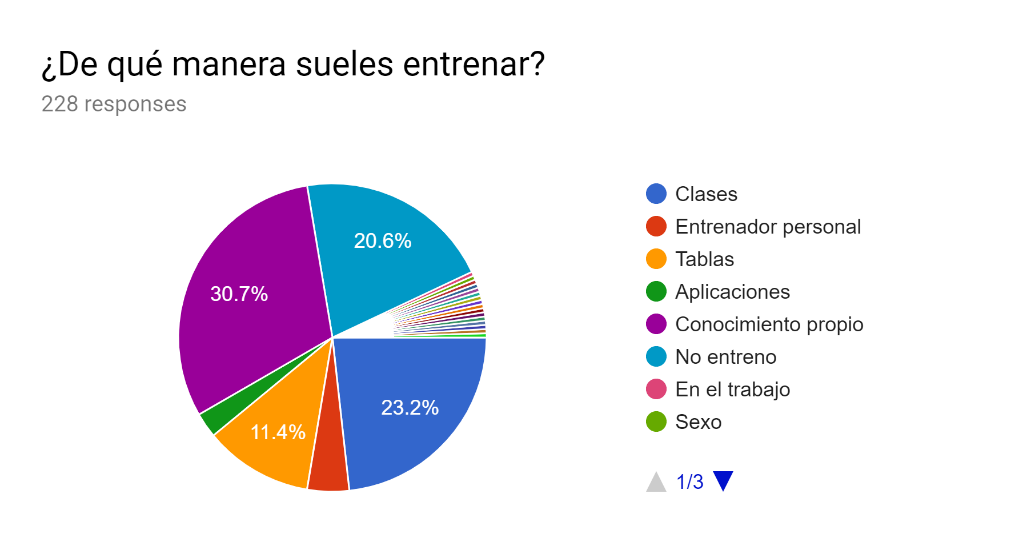
\includegraphics[scale=1]{./images/4-train-type}
		\caption{Survey: Training Type}
		\label{4_train_type}
	\end{figure}
\end{center}

The following pie represents if a personal trainer would motivate a user to go to the gym more often, this was surprising, as over 50\% would be motivated to go to the gym if they had a personal trainer guiding them and 34,2\% would maybe feel motivated to do so, after analyzing the previous graphs we consider that there is a market for a personal trainer application.

\begin{center}
	\begin{figure}[h!]
		\centering
		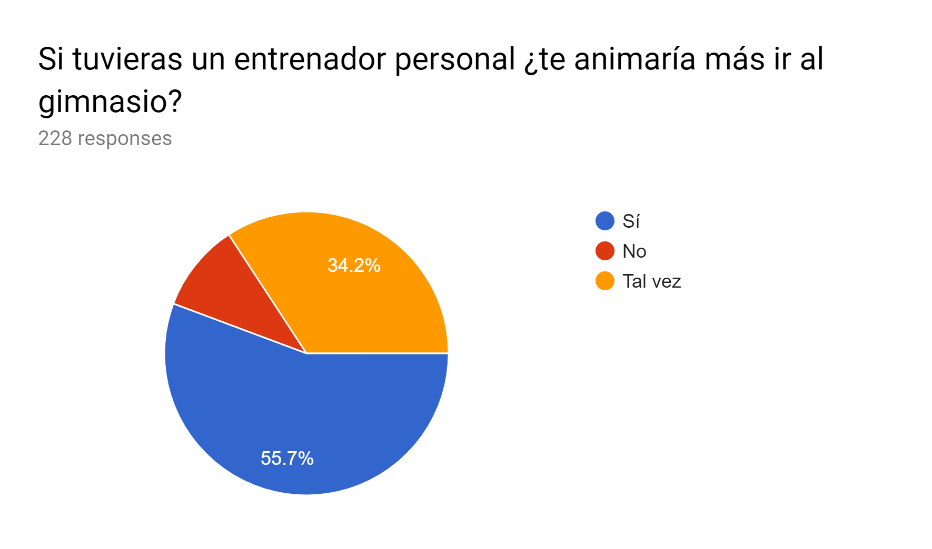
\includegraphics[scale=1]{./images/4-if-trainer}
		\caption{Survey: Having a Trainer}
		\label{4_if_trainer}
	\end{figure}
\end{center}

In the chart below we can extract some conclusions from the data, we think that 64\% of users change in some way the way they eat when they start training, but most don’t follow a strict diet. This is an important factor when developing the bot as the functionality for the recommended diets can be adapted to provide diets which tries to follow the most common eating habits of the user and slowly transition to a stricter diet, this will make users less prone to not following it.

\begin{center}
	\begin{figure}[h!]
		\centering
		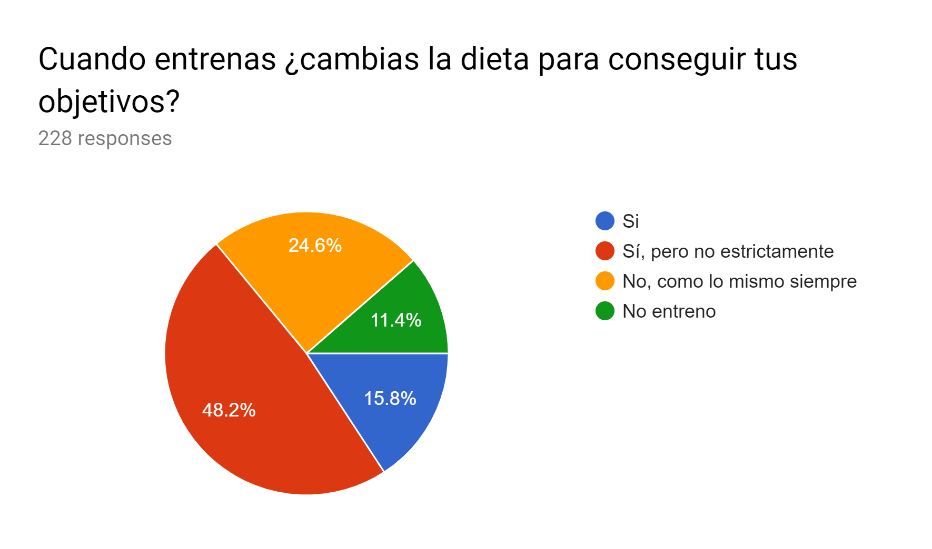
\includegraphics[scale=1]{./images/4-change-diet}
		\caption{Survey: Diet Change}
		\label{4_change_diet}
	\end{figure}
\end{center}

This graph follows up with the previous one and supports the conclusion extracted, that users rather have someone assisting with what meals to recommend the user with 84,6\% that would follow a diet recommended to them.

\begin{center}
	\begin{figure}[h!]
		\centering
		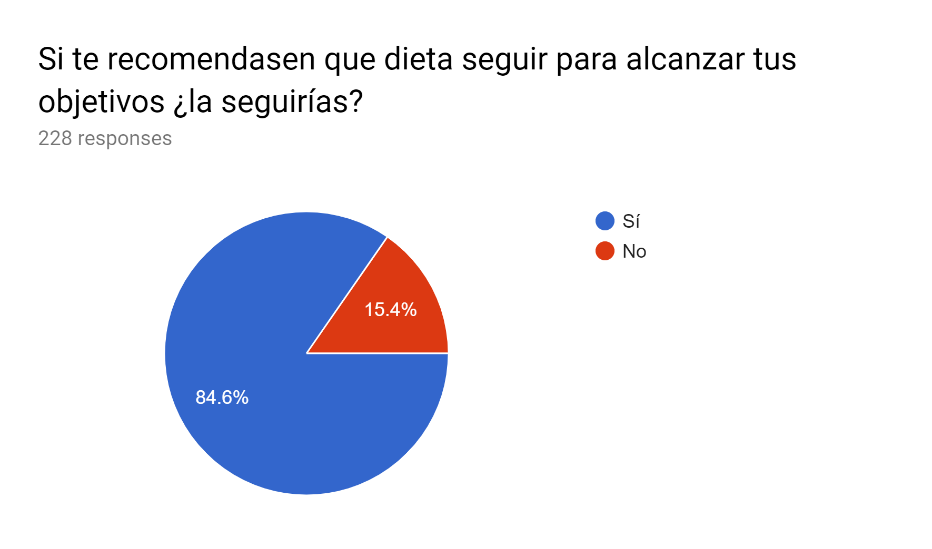
\includegraphics[scale=1]{./images/4-diet-rec}
		\caption{Survey: Diet Recommendation}
		\label{4_diet_rec}
	\end{figure}
\end{center}

The same as the previous chart in relation to exercises, the public is open and prefer someone guiding them to reach their objectives, in this case regarding exercises. This has to do with people using their own knowledge to train as compared to this graph some of the people that followed their own knowledge would rather have some one recommend what exercises to do.

\begin{center}
	\begin{figure}[h!]
		\centering
		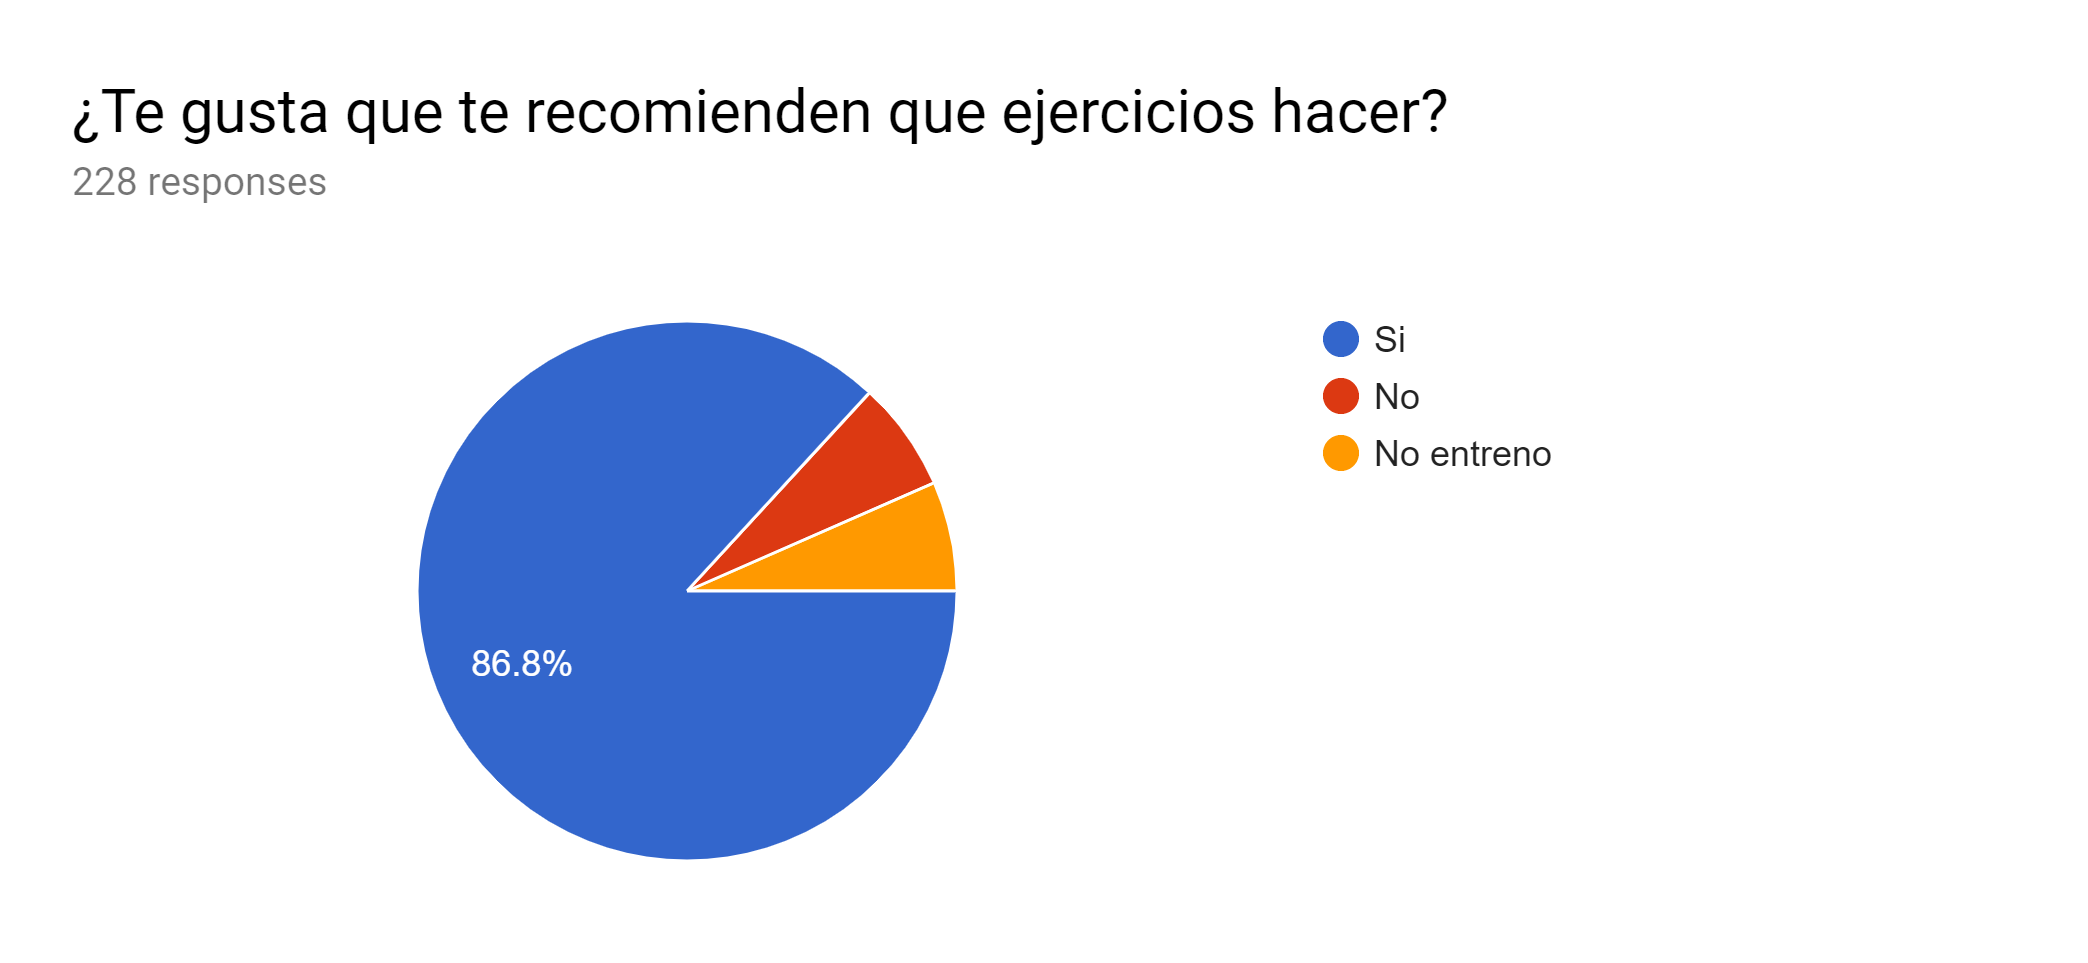
\includegraphics[scale=0.25]{./images/4-rec-exe}
		\caption{Survey: Exercise Recommendation}
		\label{4_rec_exe}
	\end{figure}
\end{center}

The most important chart of all is regarding our application, which is if these recommendations where given by a chatbot, if they would still follow it. Some curious points can be extracted from this pie, which are that most people would rather hire a professional trainer, what this tells us is that many people still prefer human contact over having a bot telling them what recommendations to follow, another point which links to a previous graph where we talked about how people train is that only 4.1\% have personal trainers, the reason being that hiring a personal trainer is costly so considering that and the fact that 35,1\% of people would follow those recommendations gives the application a large market to focus to, but also implies that the chatbot must try and simulate a human being as good as possible.

\begin{center}
	\begin{figure}[h!]
		\centering
		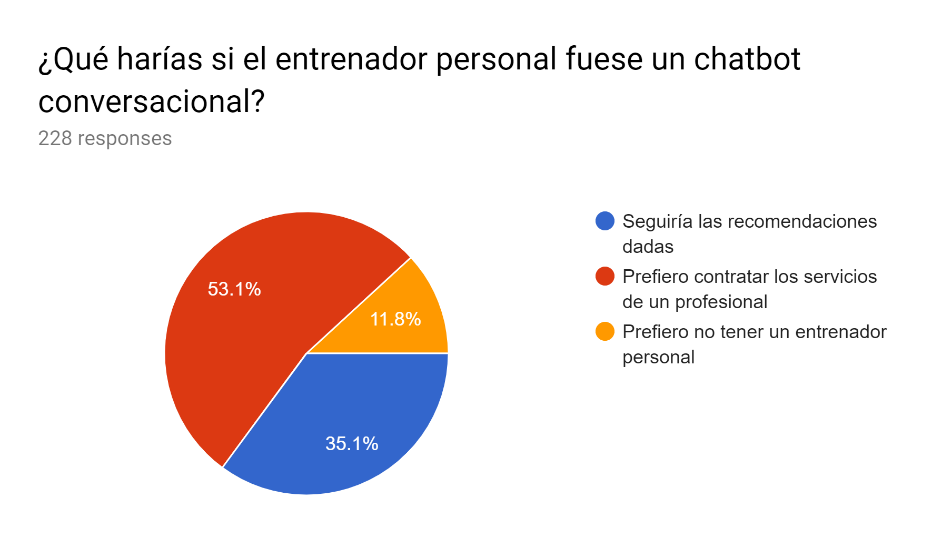
\includegraphics[scale=1]{./images/4-bot-trainer}
		\caption{Survey: Bot Trainer}
		\label{4_bot_trainer}
	\end{figure}
\end{center}

\section{Two Designs}\label{sec:chap4_design}

In this project we find that there has been two different designs, the original design was developed in a way to make the system homemade, without depending on an external platform which even though it provides a base where to start developing it limits the control the developer has in adding new functionality.\\

The second and final design does use an open source platform as the base to start developing, this had to be done because of the complexity related in developing the proprietary solution in relation to the time available to develop it. Further down the memory the reason for changing the design will be explained in more detail.

\section{Development Stages}\label{sec:chap1_dev-stag}
The project has gone though several makeovers due to the time constraint to develop the chatbot. 
\subsection{Planification}\label{sec:chap1_plan}
Originally the idea was to use a structure like a project done previously where a virtual machine in Google Cloud was the brains of the bot. In this project as there was access to a Raspberry Pi, the idea to use a cloud provider was changed to have it be the server. 
In this stage, the most time was spent on how the architecture of the bot was going to be and what technologies was going to be used throughout the project. This planning has had to be revised several times changing the whole architecture from a proprietary solution using several of the libraries mentioned before in the background to an open source platform called Rasa. Also, due to continuous problems caused by the Raspberry Pi with the installation of libraries and the lack of computing power the decision was to change the server to Azure, Microsof’s Cloud Service.
\subsection{Development}\label{sec:chap1_dev}
In this stage is where all the planning came to life and where most of the time was spent. It was composed of two plans. \\\\
\textbf{Inicial plan:}
\begin{itemize}
	\item{\textbf{Creation of a webhook to manage incoming messages from telegram in the server.}}
	\item{\textbf{DB creation to manage user info.}}
	\item{\textbf{User recognition.}}
	\item{\textbf{Intent Detection using NLTK and Scikit-learn.}}
	\item{\textbf{Conversation flows (unfinished due to complexity and time constraint).}}
\end{itemize}
\textbf{Revised plan:} \\\\
	Due to the time to create a context manager for complex conversational flows and the limit imposed by time, half way through the development it was decided to redo everything with Rasa.
\begin{itemize}
	\item{\textbf{Reconfigure webhook to manage incoming messages with rasa.}}
	\item{\textbf{Conversation stories creation.}}
	\item{\textbf{Entity extraction.}}
\end{itemize}

\section{Resources Used}\label{sec:chap1_res}
As it was said in the previous point there were two different plans, for the original one the resources used were:\\	
\begin{itemize}
	\item{\textbf{Telegram:} This was used as the platform for the user to communicate with the bot as it supports it, there are other platforms that can be used as well as integrating them isn’t complicated, but as a proof of concept telegram works well.}
	\item{\textbf{Raspberry pi:} Used as the server to hold the brains of the chatbot. Limited in computing power.}
	\item{\textbf{Python:} The programming language by excellence for machine learning as it is intuitive and has a lot of community support. The main libraries used for this original plan were:
		\begin{itemize}
			\item{\textbf{NLTK:} For the translation from human language to something the computer understands.}
			\item{\textbf{Scikit-learn:} For training and classifying the models for the bot.}
			\item{\textbf{Pickle:} To store the bot’s trained models.}
			\item{\textbf{CSV:} To load the training data from a csv file.}
		\end{itemize}	 
	}
\end{itemize}
For the revised plan a few things changed:
\begin{itemize}
\item{The Raspberry Pi was changed to a cloud solution by Microsoft called Azure, this virtual machine has double the ram of the Raspberry Pi and a higher computing power making the bot train quicker.}
\item{Even though Python is still used in this revised plan, the libraries are packaged in to the new Natural Language Engine, Rasa which takes care of training the bot.}
\end{itemize}
	
\section{Memory Structure}\label{sec:chap1_mem-str}
The document is structured in different sections where the different aspects of the project will be explained.
\begin{itemize}
	\item{\textbf{Analysis of the problem:} An in-depth analysis off the current state of the gym sector and why the need for a personal assistant is required for improving the overall efficiency when a user is working out. In this section the objectives of what this project is trying to achieve will be explained.}
	\item{\textbf{State of the art:} An analysis on how the ML and NLP technologies have evolved to the current state and where it is currently heading. What rol are chatbots taking in society.}
	\item{\textbf{Solution proposed:} How the solution provided in this project can benefit millions of people and how this project has been developed as well as the regulatory framework surrounding virtual assistants and user data manipulation.}
	\item{\textbf{Planning and budget:} How the original planning was made and how it compares to the real development. Also, this section reviews how much budget this project has taken.}
	\item{\textbf{Socioeconomic Environment:} An approach on how the current chatbot technology is changing many industries and saving costs for companies and providing a better service for their clients.}
\end{itemize}
%\begin{center}
%\begin{figure}[h!]
% \centering
%   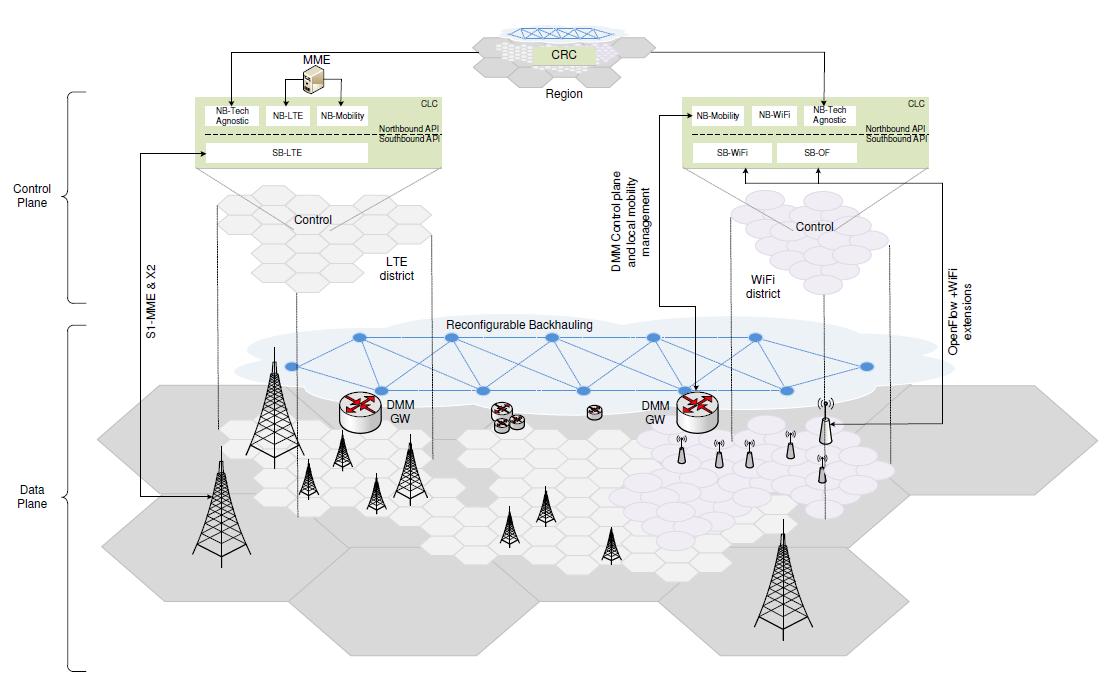
\includegraphics[scale=0.5]{./images/crowd_arch}
%	\caption{CROWD Architecture}
%	\label{crowd_arch-fig}
%\end{figure}
%\end{center}
















  	
	\chapter{State of the Art}\label{sec:chap:2}

\section{Software Defined Networking}\label{sec:chap2_sdn}

Software Defined Networking (SDN) is an approach to networking that revolves around the abstraction between the forwarding and control planes. This facilitates programmatically control over the network in order to operate network services in a deterministic, dynamic and scalable manner \cite{rfc_7426}.\\

SDN is part of a long history of efforts to make computer networks more programmable, going back more than twenty years. SDN shares simmilarities with early telephony networks, where there was a clear separation between control and data planes to simplify network management and the deployment of new services \cite{road_to_sdn}.\\

By centralizing the network control, SDN offers flexibility to congfigure, manage, secure, and optimize network resources via dynamic SDN programs that can be programed independently of the implementation of the network. SDN makes it possible to manage the entire network through intelligent orchestration \cite{new_norm_sdn}.\\

Figure 1 offers a logical representation of the SDN architecture. The Network inteligence resides in the controller, a software-based centralized SDN entity with a global view of the network. APIs between the application layer and the control layer offer the possibility of introducing applications that operate on an abstracion of the network regardless of the details of the implementation.

\begin{center}
\begin{figure}[h!]
  \centering
    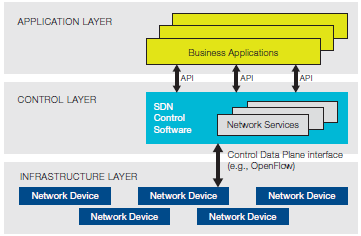
\includegraphics[scale=0.9]{./images/openflowjason}
	\caption{Openflow Logical Representation}
	\label{openflow-fig}
\end{figure}
\end{center}

\subsection{OpenFlow}\label{sec:chap2_sdn_openflow}

The Open Networking Foundation (ONF) is a non-profit organisation that is leading the development of SDN, including the standardisation of the OpenFlow protocol. OpenFlow provides the communication between the control and data planes and is the first standard interface designed specifically for SDN. Some of the benefits OpenFlow-based SDN offer to enterprises and carriers are:

\begin{itemize}
\item{\textbf{Centralized management and control of multi-vendor environments:} SDN control software can control any OpenFlow-enabled device.}
\item{\textbf{Reduced complexity through automation:} OpenFlow-based SDN offers a flexible network automation and management framework.}
\item{\textbf{Higher rate of innovation:} Due to the capacity of network operators to program te network in real time to meet specific needs in a short frame of time.}
\item{\textbf{Increased network reliability and security:} Due to the complete visibility and control of the network from a centralized entity.}
\item{\textbf{More granular network control:} Capability of setting low level network parameters at a high level.}
\item{\textbf{Better end-user experience:} Due to network behaviour adapting to the user's needs, using state information being available to higher-level applications.}
\end{itemize}

Both the SDN controller and the network nodes run the OpenFlow protocol. The OpenFlow protocol's key concept are flows, which identify the network traffic based on rules that are programmed at the SDN control level. These rules establish the way traffic flows through the network through the diffent network nodes that form it.

\subsubsection{OpenFlow Switch}\label{sec:chap2_sdn_openflow_switch}

An OpenFlow Switch is a software program or hardware device that consists at least of a Flow Table, an Action associated with each Flow Table Entry and an OpenFlow Secure Channel. The Flow Table performs packet lookups and forwarding, and the OpenFlow Secure Channel connects the OpenFlow switch with the SDN Controller. The switch communicates with the controller and the controllwer manges the switch via the OpenFlow protocol \cite{of_switch_spec}. Figure \ref{openflowswitch-fig} depicts a logical view of the OpenFlow Switch.\\

A high percentage of today's routers and Ethernet switches run flow-tables that are usually built from TCAMs, and OpenFlow takes advantage of common functionalities they share. Exploiting this feature, the OpenFlow protocol can program the flowtable regardless of the vendor of the equipment \cite{of_campus_net}.

\begin{center}
\begin{figure}[h!]
  \centering
    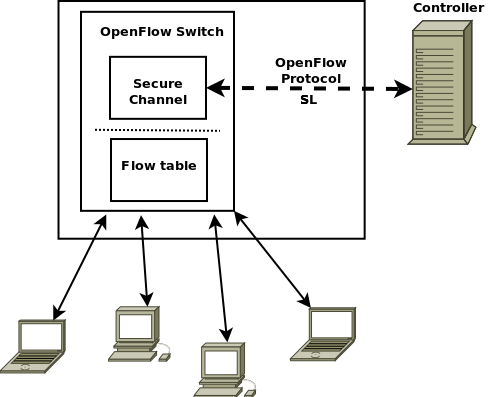
\includegraphics[scale=0.55]{./images/OpenFlowSwitch}
	\caption{OpenFlow Switch Representation}
	\label{openflowswitch-fig}
\end{figure}
\end{center}

The datapath of an OpenFlow Switch consists of a Flow Table containing three fields:

\begin{itemize}
\item{\textbf{Packet header:} Defines the flow.}
\item{\textbf{Action:} Defines how the flow should be processed.} 
\item{\textbf{Statistics:} Keeps track of the number of packets and bytes introduced by the flow and how long since the last packet for control of inactive flows.}
\end{itemize}

The three basic actions to be included in the action field of a Flow Table are:

\begin{itemize}
\item{\textbf{Forward:} In order to provide routing capabilities, this action forward packets associated to a given flow to a port or group of ports.}
\item{\textbf{Encapsulate:} This encapsulates a packet of a given flow (typically only the first packet) and sends it to the SDN controller for processing. The controller must decide if the flow should be added to the Flow Table.} 
\item{\textbf{Drop:} This commands to drop packets from a given flow. }
\end{itemize}

\section{Distrbuted Mobility Management}\label{sec:chap2_dmm}

Distributed mobility management (DMM) is an alternative to centralized mobility protocols such as Mobile IPv6, Hierarchical Mobile IPv6 and Proxy Mobile IPv6. The IETF is leading the standardization of DMM solutions. The DMM working group 
\footnote{\url{http://datatracker.ietf.org/wg/dmm/}} was formed in March 2012 to address the need for the implementation of a distributed anchoring model in mobile networks. The motivation to study and develop the DMM arquitectural paradigm resides in the following two challenges \cite{rfc_7333}: 

\begin{itemize}
\item{Mobile access to the Internet is increasing drastically. The traffic this will generate creates the need for updated requirements for data traffic delivery in mobile core networks. The ``flattening'' of mobile networks proves to work best for direct communication between closely located peers.}
\item{A study on mobility patterns suggest mobile nodes remain attached to the same point of attachment for relatively long periods of time \cite{locating_user}. IP mobility support is currently designed to always be active, resulting in an unnecessary loss of costs and resources.}
\end{itemize}

In centralized mobility management, the session and forwarding information is kept in a single centralized mobility anchor, which is in charge of forwarding the traffic to the mobile node's current location. The DMM arquitecture suggests a flat access by means of the distribution of mobility anchors in the data plane so that they are positioned nearer to the user. This optimises state information management because it avoids unnecessary mechanisms to forward traffic from an old mobility anchor to a new mobility anchor.\\

Problems that are solved with a DMM implementation are:

\begin{itemize}
\item{\textbf{Sub-optimal routes:} Since mobility anchors are fixed at the home address, this is where all traffic will arrive and must be forwarded from to the current mobile node's address. This results in longer end-to-end paths meaning higer delays. With a distributes mobility architecture, as the anchors are located at the very edge of the network, close to the user terminal, data paths tend to be shorter \cite{fama}.}
\item{\textbf{Lack of scalability:} A centralized entity in charge of maintaining mobility context information for each mobile node needs to have enough processing and routing capabilities to deal with all the mobile users' traffic simultaneously. DMM sugests distributing the load among several network entities.} 
\item{\textbf{Divergenge from network trends:} Mobile networks have an evolutionary tendency to become flatter, contrary to the approach of centralized mobility management}
\item{\textbf{Single point of failure and attack:} A centralized entity in charge of maintaining mobility context information for each mobile node means there is a unique point of failure and attack.}
\item{\textbf{Unnecessary mobility support:} IP mobility support is usually provided to all mobile nodes, even for users that will not move from the first point of attachment. This also applies to sessions that deal with mobility at an application level or applications that don't need a stable IP address during a handover to maintain session continuity.}
\end{itemize}

The two main approaches to implementing Distributed Mobility Management architectures in modern wireless networks are, on one side, transforming Mobile IPv6 into a distribution-oriented protocol, and, on the other, doing the same for Proxy IPv6. These approaches can be identified as client-based or network-based solutions respectively \cite{dmm_standard_land}:

\begin{itemize}
\item{\textbf{Client-based solution:} Based on the Mobile IPv6 protocol, this solution involves deploying multiple home agents at the edge of the network in order to distribute the mobility anchors. This is achieved through the idea that a mobile node can have assigned more than one IP address, meaning that the mobile node can have assigned a new IP address every time it visits an access network.}
\item{\textbf{Network-based solution:} Based on the Proxy IPv6 protocol, this solution suggests moving the mobility anchors to the edge of the network, and give them the capability for managing both the control and data plane seperately. The ability of managing both planes seperately offers the possibilty for optimal routing of data traffic.} 
\end{itemize}

\subsection{Mobile IPv6}\label{sec:chap2_dmm_mip}

Mobile IPv6 is a protocol that provides mobility support offering capabilities to mobile nodes so they can move from one Access Point to another without changing the mobile node's home address, the mobile node's permanent address. Without mobility support, once the mobile node leaves the home link, where the mobile node has its subnet prefix assigned (the first point of attachment), packets could not find there way to the mobile node. 

\subsubsection{Basic Operation}\label{sec:chap2_dmm_mip_bo}

\begin{center}
\begin{figure}[h!]
  \centering
    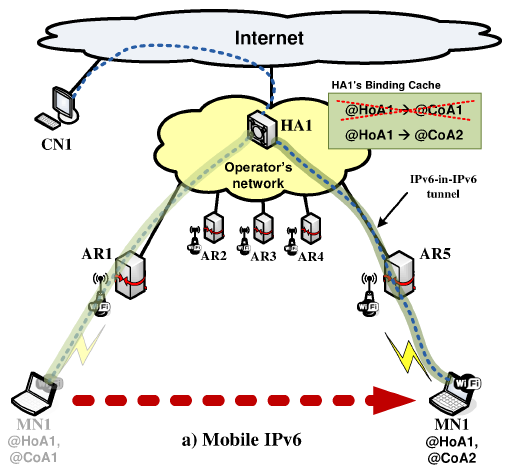
\includegraphics[scale=0.3]{./images/mip}
	\caption{Mobile IP}
	\label{mip-fig}
\end{figure}
\end{center}

More detailed information regarding the basic operation of this protocol be found in \cite{rfc_6275}.

\subsection{Proxy Mobile IPv6}\label{sec:chap2_dmm_pmip}

Mobile IPv6 poses the problem of needing the involvement of the client, having to exchange signaling messages with the home agent in order to inform of the mobile node's new location so that the home agent can redirect traffic. The Proxy Mobile IPv6 approach is a Network-based one, excluding the involvement of the host. This is possible thanks to a new entity called proxy mobility agent, that is in charge of the communication with the home agent and manange the mobility on behalf of the client.

\subsubsection{Basic Operation}\label{sec:chap2_dmm_pip_bo}

\begin{center}
\begin{figure}[h!]
  \centering
    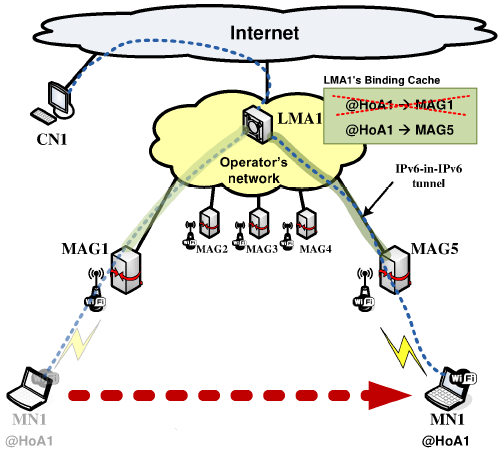
\includegraphics[scale=0.3]{./images/pmip}
	\caption{Proxy Mobile IP}
	\label{pmip-fig}
\end{figure}
\end{center}

More detailed information regarding the basic operation of this protocol be found in \cite{rfc_5213}.


\section{LTE}\label{sec:chap2_lte}

The Long Term Evolution of UMTS is the result of great technological advances in mobile telecommunications systems,standardized within the 3GPP (3\textsuperscript{rd} Generation Parnership Project) as part of the 3GPP Release 8 feature set. After the developement and standardization of GSM (Global System for Mobile communications) belonging to the 2G family, 3G  Universal Mobile Telecommunications System (UMTS) came after with the entry of Code Division Multiple Access into the 3GPP evolution track, known as Wideband CDMA (WCDMA). This technology evolved until the arrival of LTE and the adoption of Orthogonal Frequency-Division Multiplexing (OFDM), which is the access technology dominating the latest evolutions of all mobile radio standards \cite{lte_history}.\\

The LTE access network is a network of base stations called evolved NodeB (eNB), generating a flat architecture, and is the access part of the Evolved Packet System (EPS) Figure \ref{lte_arch-fig}.

\begin{center}
\begin{figure}[h!]
  \centering
    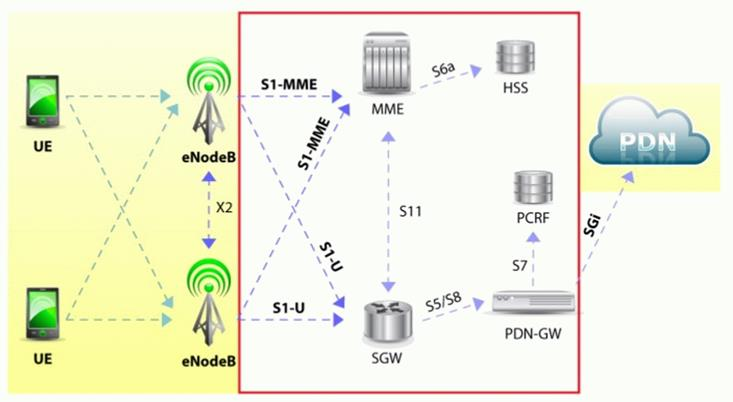
\includegraphics[scale=0.7]{./images/lte_arch}
	\caption{LTE Architecture}
	\label{lte_arch-fig}
\end{figure}
\end{center}

The latest advancements in LTE technology involve \cite{lte_wp}:

\begin{itemize}
\item{\textbf{Small Cell Enhancements}: Higher Order Modulation (256QAM) and Dual connectivity for LTE.}
\item{\textbf{Device to Device communication (D2D)}: Offerening direct and group communication between terminals.}
\item{\textbf{WLAN/3GPP Radio Internetworking}: Integration of WLAN access capabilities into  the data transfer.}
\item{\textbf{HetNet mobility enhancements}: Enhance the capacity of a cellular network by introducing heterogeneous networks (HetNets) improving overall handover performance and robustness.}
\item{\textbf{Smart Congestion Mitigation (SCM)}: For congestion control.}
\end{itemize}

\subsection{LTE emulation}\label{sec:chap2_lte_emu}

LTE emulation can be perfomed with a combination of ns-3, a discrete event network simulator used to create an open simulation environment for computer networking research and NI PXI systems \cite{ni_pxi_wp} (Figure \ref{pxi-fig}).

\begin{center}
\begin{figure}[h!]
  \centering
    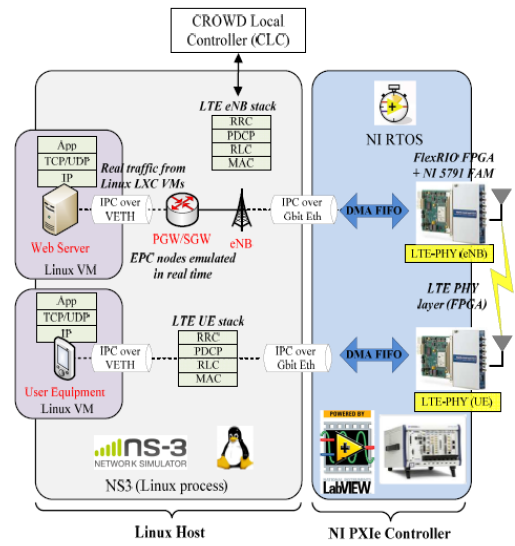
\includegraphics[scale=0.7]{./images/pxi}
	\caption{LTE emulation with ns-3 and NI PXI}
	\label{pxi-fig}
\end{figure}
\end{center}

\subsubsection{NI PXI}\label{sec:chap2_lte_emu_pxi}

PXI is a rugged PC-based platform for measurement and automation systems. PXI combines PCI electrical-bus features with the modular, Eurocard packaging of CompactPCI and then adds specialized synchronization buses and key software features. PXI is both a high-performance and low-cost deployment platform for applications such as manufacturing test, military and aerospace, machine monitoring, automotive, and industrial test. Developed in 1997 and launched in 1998, PXI is an open industry standard governed by the PXI Systems Alliance (PXISA), a group of more than 70 companies chartered to promote the PXI standard, ensure interoperability, and maintain the PXI specification \cite{ni_pxi_whatis}.

\subsubsection{ns-3}\label{sec:chap2_lte_emu_ns3}

ns-3 is a discrete-event network simulator, targeted primarily for research and educational use. ns-3 is free software, licensed under the GNU GPLv2 license, and is publicly available for research, development, and use.
The goal of the ns-3 project is to develop a preferred, open simulation environment for networking research: it should be aligned with the simulation needs of modern networking research and should encourage community contribution, peer review, and validation of the software \cite{ns3_whatis}.

















	\chapter{Analysis Of The Problem}\label{sec:chap:3}

The number of mobile users is increasing dramatically, translating into an increasing demand of mobile data services. Mobile data traffic increased by 81\% in 2013 and by 69\% in 2014 \cite{internet_trends} and the rate of increase is not slowing down. 5G, the mmWave, is disruptive upcoming technology that employs frequencies in the order of 60GHz that will impose very high requirements, given the extremely high bandwidths it will provide in very small areas \cite{5g}. This has a direct correlation with both the increased accesibility to the internet from mobile devices via WLANs and RANs, and the increase in popularity of applications designed for smartphones and tablets. On top of this, operators are migrating their networks to full IP based networks for both voice and data \cite{fama}.

\begin{center}
\begin{figure}[h!]
  \centering
    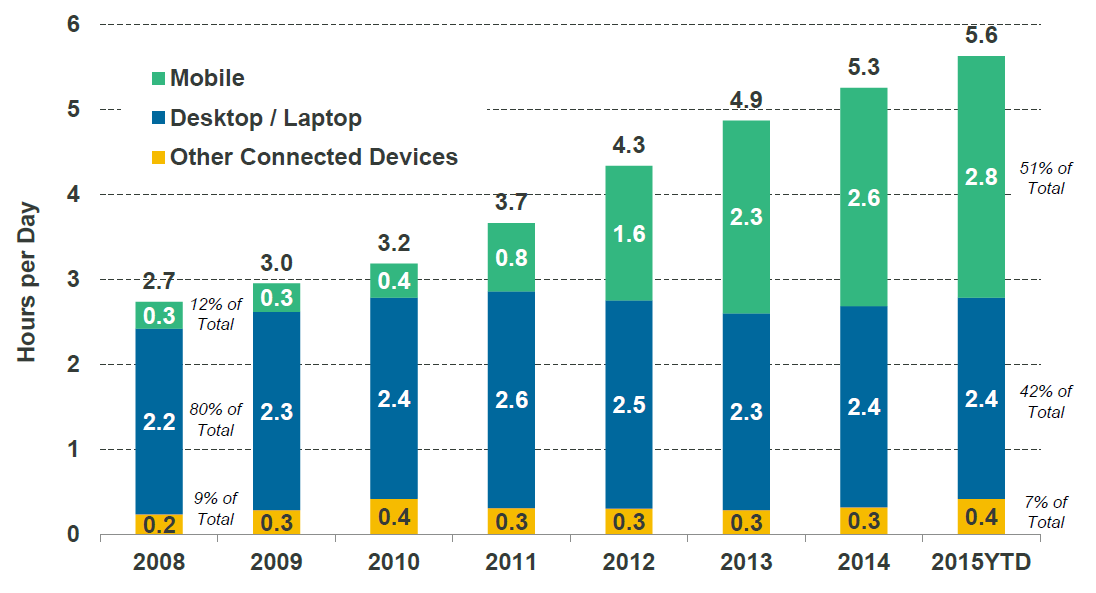
\includegraphics[scale=0.4]{./images/traffic_data}
	\caption{Mobile Traffic Data}
	\label{traffic_data-fig}
\end{figure}
\end{center}

Current centralized mobility management solutions include protocols such as Mobile IPv6 or Proxy Mobile IPv6. These protocols depend on a centralized entity for mobility management and data forwarding. This makes these solutions vulnerable to problems such as:

\begin{itemize}
\item{\textbf{Sub-optimal routing}}
\item{\textbf{Scalability}}
\item{\textbf{Signaling overhead}}
\item{\textbf{Complex network deployment}}
\item{\textbf{Lake of granular network control}}
\item{\textbf{Single point of failure}}
\end{itemize}

On the other hand, interference due to uncoordinated resource sharing techniques reprensents a key limiting factor in the design of dense wireless networks \cite{sdn_dense}.\\

The solution proposed in this project is a combination of Software Defined Networking and Distribted Mobility Management to tackle these problems.










	
	\chapter{Solution Proposed}\label{chap:4}

\section{Architecture}\label{sec:chap4_arch}

[INSERT FIGURE OF ARCHITECTURE]

\subsection{Hardware}\label{sec:chap4_arch_hard}

\subsection{Software}\label{sec:chap4_arch_soft}

\section{Network-Based Mobility Solution}\label{sec:chap4_net_based}

\subsection{Attachment}\label{sec:chap4_net_based_attach}

\subsection{Start video}\label{sec:chap4_net_based_video}

\subsection{Intradistrict handover}\label{sec:chap4_net_based_intra}

\subsection{Interdistrict handover}\label{sec:chap4_net_based_inter}

\section{Host-Based Mobility Solution with LTE emulation}\label{sec:chap4_host_based}

\subsection{Handover to LTE district}\label{sec:chap4_host_based_lte}

\section{On-demand Infrastructure}\label{sec:chap4_ondemand}

\subsection{Switching off an Access Point}\label{sec:chap4_host_based_lte}

\subsection{Switching on an Access Point}\label{sec:chap4_host_based_lte}




	\chapter{Implementation}\label{chap:5}


	\chapter{Design Alternatives}\label{chap:6}

\section{CROWD Controller hardware}\label{sec:chap6_ctrl}

The CROWD Local Controllers and the CROWD Regional Controllers were originally Linux personal computers. These were replaced by single-board computers called Minnowboard. The Minnowboard offered the possibility of having its higher processing resources dedicated exclusively to the Controller functions. Being much smaller in size, they are much easier to transport and to set up. On top of this, they offered HDMI capabilities, contrary to their pc counterpart. More information about the Minnowboard can be found in Chapter \ref{sec:chap4_arch_hard}.

\section{LTE emulation tool}\label{sec:chap6_lte}

LTE emulation could be perfomed with either ns-3, a discrete event network simulator used to create an open simulation environment for computer networking research, or with a combination with ns3 and NI PXIe systems (a detailed description of each solution can be found in Chapter \ref{sec:chap2_lte_emu}. While ns-3 + NI PXIe systems offered the most realistic results, due to using real non-emulated transceivers for data transmission and reception, the NI PXIe systems are very expensive, hard to transport, hard to set-up, and not always available to use.

\section{On-demand infrastructure switch off mechanism}\label{sec:chap6_switch}

The mechanism used for switching off Access Points has the drawback of doing so in an aggresive manner, meaning the Access Points are switched off directly cutting the electric power. This is a solution limitation that does not have a major impact, so an alternative has not been taken into consideration.

\section{Access point hardware}\label{sec:chap6_ap}

The options at hand were either using Linksys routers for the Access Points, or using an Alix board. The decision of choosing the Alix board instead of the Lynksis router was weighing the limitation of the Linksys router which is that it can't run the linux distribution needed, against the drawback of the Alix board that is the long time it takes to start up when switched off.

	
	\chapter{Experiments}\label{sec:chap:7}


	\chapter{Planning}\label{chap:8}

	
	\chapter{Regulatory Framework}\label{chap:9}



	\chapter{Socio-Economic Environment}\label{chap:10}



	\chapter{Conclusions}\label{chap:11}



	\chapter{Summary}\label{chap:12}


	
	\bibliographystyle{ieeetr}
\bibliography{main}

		
	\appendix

	


\end{document}
